% Set document properties as required by FEKT specification
\documentclass[a4paper, 12pt]{article}
\usepackage[left=3cm,right=2cm,top=4cm]{geometry}

% Local settings
\usepackage[utf8x]{inputenc} 
\usepackage[czech]{babel}
\usepackage[IL2]{fontenc}
\usepackage{afterpage}
\usepackage{amsthm}
\usepackage{graphicx}
\usepackage{amsmath}
\usepackage{amsfonts}
\usepackage{fancyvrb}
\usepackage{hyperref}
\usepackage{pdfpages}
\hypersetup{
    colorlinks,
    citecolor=black,
    filecolor=black,
    linkcolor=black,
    urlcolor=black
}

% Set line spacing for whole document (sadly)
\renewcommand{\baselinestretch}{1.5}

% Helper commands
\providecommand{\uv}[1]{\quotedblbase #1\textquotedblleft}
\newcommand\textbox[1]{%
    \parbox{.5\textwidth}{#1}%
}

% Thesis variables
\newcommand{\thesisName}{Implementace kybernetické bezpečnosti do ŠVP pro Informatiku a výpočetní techniku na gymnáziích}
\newcommand{\universityName}{VYSOKÉ~~~UČENÍ~~~TECHNICKÉ~~~V~BRNĚ}
\newcommand{\facultyName}{Fakulta elektrotechniky a komunikačních technologií}
\title{\thesisname}
\author{Bc. Daniel Dušek}

% === WORK TODO LIST ===
%
% PRAKTICKÁ ČÁST - TÉMATA, OSNOVY
% Hodina 3: Bezpečnost na Internetu (mohla by být řazena jako druhá, za Identitu)
% Hodina 4:  
%
% Source from mail: ICT zavedena v rámci nějaké konkrétní vllnovité implementace


\begin{document}

% === FRONT PAGE ===
\thispagestyle{empty}
\newgeometry{left=2cm,right=2cm,top=1.5cm}
    \begin{center}
        \Huge
        \universityName \\
            \vspace{\stretch{0.150}}
        
        \LARGE
        \textsc{\facultyName\\}
            \vspace{\stretch{0.300}}
        
        \Large{Závěrečná práce doplňujícího pedagogického studia \\ ~ \\}
        
        \LARGE
        \textsc{\thesisName}
            \vspace{\stretch{0.618}}
    \end{center}

        % Author and date part        
        \noindent \textbox{\today}  \textbox{\hfill \textbf{Vedoucí práce}: PhDr. Petra Fiľová} \\
        \noindent \textbox{\hfill}  \textbox{\hfill \textbf{Autor práce}: Bc. Daniel Dušek ~~~~~}
\clearpage
\restoregeometry

% === TABLE OF CONTENTS ===
% Potential TODO: NO line spacing as well?
\newpage
\thispagestyle{empty}
\tableofcontents

% === SECTION INTRODUCTION ===
\newpage
\setcounter{page}{1}
\section{Úvod}

Stejně jako bylo devatenácté století nazývané stoletím páry a dvacáté století stoletím techniky, bude jednou pravděpodobně dvacáté první století nazývané stoletím počítačů a sítí. Oblast techniky a informačních technologií se rozvíjí neustále vyšší a vyšší rychlostí, dostupnost \uv{chytré} elektroniky se zvyšuje tempem podobným. Společně s technikou a její vyšší dostupností se však objevuje další, bohužel nepříjemný fenomén -- a sice zneužívání technologií a jejich vysoké dostupnosti k páchání trestné činnosti. 

Trend zneužívání technologií a nedostatečné vzdělanosti v oblasti počítačové bezpečnosti lidí s nimi pracujících roste s každým rokem více a více. Útoky související s distribucí, v době psaní práce velmi populárního škodlivého software, zvaného ransomware vzrostly v počtu od roku 2015 neuvěřitelných 300$\%$.

Na jednu stranu možná i uklidňujícím faktem je, že v případě ransomware jsou cílem typicky organizace, nikoliv jednotlivci. Bohužel i v tomto případě se často obětí stane právě i jednotlivec, a to zejména díky způsobu, kterým se ransomware a jemu podobné škodlivé programy šíří. Jedním z častých scénářů je případ, kdy je počítač infikován prostřednictvím nakaženého souboru typu .xls(x), .doc(x), .ppt(x) apod., tedy soubory běžně produkované nástroji sady Microsoft Office. Druhým, opět velmi častým scénářem je pak případ, kdy se škodlivý soubor pouze tváří být souborem dříve jmenovaných typů, avšak ve skutečnosti je souborem úplně jiného typu, obsahujícího škodlivý kód. V obou dvou scénářích je klíčové, aby ovšem pochybil lidský článek pracující s takovýmto souborem. Tomuto pochybení by bylo poměrně snadné předcházet, a to vyšším obecným povědomím o tom jak správně a bezpečně pracovat s počítačem a internetem. 

Tohoto obecně vyššího povědomí by bylo možné dosáhnout například kladením vyššího důrazu na výuku kybernetické bezpečnosti ve školách v rámci výuky informačních technologií, výpočetní techniky a informatiky. V konkrétních termínech například místo kladení obrovského důrazu pouze na výuku práce s nástroji kancelářského balíku Microsoft Office slevit lehce z časové dotace vyhrazené na vysvětlování funkcionality a následné zkoušení žáků z ní, a tuto časovou úsporu věnovat k osvětlování způsobů a principů, kterými jsou soubory balíku Microsoft Office zneužívány hackery pro napadení počítačů a způsobů obrany a bezpečné práce s těmito soubory. Snížení časové dotace na vysvětlování a zkoušení funkcionality by, dle autora této práce, nemuselo mít vyloženě negativní dopad, neboť většina dnešní generace přichází do styku s počítači a těmito programy na denní bázi. Navíc jsou tyto programy v posledních letech průběžně neustále vylepšovány z hlediska uživatelské přívětivosti, aby práce s nimi byla více intuitivní a snadná. 

Dalším důvodem pro zavedení výuky kybernetické bezpečnosti do osnov je zcela opačný pól kybernetické bezpečnosti. Doposud bylo psáno hlavně o způsobech ochrany a osvěty běžných uživatelů výpočetní techniky proti útokům ze strany hackerů. Stejně, ne-li více důležitou částí výuky kybernetické bezpečnosti by měla být osvěta žáků o možných následcích zneužívání výpočetní techniky k páchání trestných činů. Mezi studenty se vyskytuje dnes již poměrně veliká část žáků, která je seznámena s prací s počítačem natolik, že je potenciálně schopná počítač i nějakým způsobem programovat. Někteří z těchto žáků mohou potřebovat vyjasnit fakt, že existuje hranice, za níž nesmí při programování svých aplikací zajít. Ačkoliv se to může zdát z prvního pohledu jako celkem jednoduchá otázka k diskusi, nemusí to vždy být pravda. Konkrétním případem může být 16 letý chlapec Ashkan Hosseini, jenž naprogramoval aplikaci, kterou nahrál na CD s rodinnými fotkami~\cite{malwareUnicornAppretince}. Aplikace následně způsobila, že po strčení CD do počítače došlo k vymazání všech rodinných fotek jak z CD, tak z počítače, do kterého bylo CD zastrčeno. Ashkan naprogramoval tuto aplikaci za účelem odstranění fotek na kterých se nacházel -- jeho úmysly tedy nebyly vyloženě špatné a díky tomu, že CD putovalo pouze mezi rodinou, Ashkan nebyl nikým žalován. Pokud by se ale stalo, že by jeho aplikace unikla do světa a napadla cizí počítač, dopustil by se již vážného trestného činu, aniž by si tyto následky svých akcí uvědomil. V Americe by to pro něho pak mohlo znamenat až 5 let vězení. Příběh Ashkana Hosseiniho dopadl tedy naštěstí pro něho dobře, kde navíc jeho rodiče měli dostatek reflexe a nabídli mu možnost studovat oblast boje proti kybernetické kriminalitě, které se chopil. Ne všichni žáci však musí vždy přesně odlišit hranici toho, kdy končí \uv{legrace} a začíná páchání trestného činu, alespoň ne v oblasti počítačů a sítí, a ne všichni musí mít to štěstí, jaké Ashkan měl. I z tohoto důvodu je třeba šířit povědomí o kybernetické bezpečnosti a implikacích, které může mít na život jedince nedodržování jejích zásad. 

V letech 2007--2009 byla reakcí českého školství na prudký rozvoj a expanzi výpočetní techniky snaha naučit žáky a studenty s těmito novými technologiemi pracovat a interagovat. Tato snaha byla realizována v rámci vlnově vydávaných rámcově vzdělávacích programů -- dále jen RVP -- v nichž byl již povinně vyhrazen prostor pro výuku informačních a komunikačních technologií a informatiky~\cite{waveRVP}. Autor této práce považuje tuto reakci za dobře načasovanou a vhodnou. 

Nyní však nastává nová éra, kdy zařízení schopná připojení k Internetu jsou doslova i obrazně na každém našem kroku. Každé zařízení připojené k Internetu se může stát cílem útoku, stejně jako se obětí počítačové kriminality může stát každá osoba s těmito zařízeními pracující. Vzniká tedy takto nová potřeba většího důrazu na výuku těchto aspektů práce s informačními technologiemi. Tato práce má za cíl demonstrovat konkrétní možnou implementaci takové výuky do výuky ICT na gymnáziích.

% === DICTIONARY ===
% TODO: Zkontrolovat, že všechna problematická slova se vyskytují ve slovníčku pojmů.
\newpage
\section{Slovníček pojmů}
V textu této práce je možné se setkat s pojmy, které mají speciální význam v oblasti počítačové či kybernetické bezpečnosti, jenž se často liší od pocitového významu, který by si oblasti neznalý čtenář mohl vytvořit. Tato sekce si klade za cíl rozptýlit možné nejasnosti a mnohoznačnosti.

\textbf{Malware} -- Souhrné označení pro programy které vykonávají škodlivou činnost (trojské koně, viry, programy špehující uživatele, programy zobrazující uživateli nevyžádanou reklamu, a další).

\textbf{Škodlivý kód} -- Chce-li programátor přikázat počítači, aby vykonal nějakou činnost, popíše tuto činnost pomocí tzv. \textit{kódu}. Škodlivý kód je pak takový kód, který je-li vykonán počítačem, provede něco, co uživatel/majitel tohoto počítače nechce. Útočníci se při útoku snaží typicky právě vykonat škodlivý kód na zařízení, které napadají. Tento škodlivý kód bývá velmi často nastražen a ukryt tak, aby si uživatel pracující s počítačem vůbec neuvědomil, že kód spouští a vykonává.

\textbf{Nakažený soubor} -- Soubor v němž je kromě původního obsahu souboru navíc obsažen škodlivý kód. Škodlivý kód do souboru umístil buď přímo, nebo zprostředkovaně (například prostřednictvím škodlivého programu) útočník.

\textbf{Ransomware} -- Škodlivý program založený na principu držení rukojmí. Program po průniku do počítače zašifruje některé soubory, popřípadě uživateli úplně znemožní práci s počítačem. Za zpřístupnění souborů či zařízení je po uživateli požadováno zaplacení výkupného. Zaplacení výkupného nemusí vždy vést k získání objektu, který je držen jako rukojmí.

\textbf{Phishing} -- Typ útoku při kterém útočník předstírá, že je důvěryhodná, uživateli dobře známá entita, aby uživatele přiměl k vydání osobních či jinak citlivých informací a dat.


% === RVP & SVP CHAPTER ===
% Doslova z papíru: Kap. RVP, ŠVP konkrétní školy - Informace - počet hodin / týden, Skoro kopie RVP/ŠVP s rozborem
\newpage
\section{Výuka informatiky dle Rámcového Vzdělávacího Programu a Školního Vzdělávacího Programu}
Tato část práce se zabývá prostorem vyhrazeným pro výuku informatiky v rámci Rámcového Vzdělávacího Programu (dále jen RVP) a jeho možnou utilizací pro výuku kybernetické bezpečnosti. Dále je zde rozebrán konkrétní Školní Vzdělávací Program (dále jen ŠVP) v rámci něhož je vyhrazen prostor pro výuku informatiky. Jsou zde také zmíněny očekávané výstupní dovednosti, kterými by student po absolvování vyučování informatiky měl disponovat.
%Bez dalších poznámek, pravděpodobně půjde o rozbor toho co mi bude k dispozici (pokud nezískám ŠVP, asi se pustím do počtu hodin z RVP a zkusím vygooglit ŠVP nějaké školy, co to má veřejně). Patří sem informace o ŠVP/RVP, počet hodin na týden.

% === PREREQUISITIES ===
\newpage
% TODO: Ocitovat RVP pro gymnázia & RVP pro základní školy
% TODO: Přijít na to jak správně pojmenovat kapitolu "Vstupní dovednosti"
% Očekávané výstupy – 1. a 2. období (základní vzdělávání)
% žák
% ICT-5-1-01 využívá základní standardní funkce počítače a jeho nejběžnější periferie
% ICT-5-1-02 respektuje pravidla bezpečné práce s hardwarem i softwarem a postupuje
%   poučeně v případě jejich závady
% ICT-5-1-03 chrání data před poškozením, ztrátou a zneužitím
\section{Vstupní dovednosti}
V této části práce jsou vymezeny vstupní dovednosti, kterými by studenti pro úspěšnou výuku kybernetické bezpečnosti měli disponovat. Dále je zde navrženo a argumentováno časové zasazení výuky napříč ročníky, pokryty jsou také možné formy výuky vhodné pro předmět kybernetické bezpečnosti a nezbytné pomůcky pro kvalitní výuku.
% Osnova
% * Vstupní dovednosti
% * Pomůcky pro výuku - u počítačů specifikovat operační systém, HW, to samé pro telefony, náhradní řešení bez telefonů
% * Časový rozvrh napříč ročníky
% * Formy výuky 
%           Bodově z konzultace: předpokládané vstupní dovednosti, ve kterých ročnících by se to mělo vyučovat (předběžně domluveno na všechny), probrat možné formy výuky (výklad, exkurze, protip: přivedení člověka odsouzeného za trestnou 
%           činnost (část s vysvětlováním právní závadnosti)), potřebné pomůcky pro realizaci: jak výkonné musí být počítače, jaké by měly být jejich parametry (asi internet je třeba), jde využít telefony (jak?), interaktivní tabule

\subsection{Vstupní dovednosti}
Text vstupních dovedností.

\subsection{Pomůcky pro výuku}
Test pomůcek ve výuce.

\subsection{Časový rozvrh napříč ročníky}
Text časového rozvrhu napříč ročníky

\subsection{Formy výuky}
Způsobů a forem, kterými lze vyučovat a demonstrovat kybernetickou bezpečnost by se jistě dalo vymyslet mnoho. Zde jsou shrnuty formy výuky, které autor práce považuje za efektivní a vhodné v oblasti kybernetické bezpečnosti, společně s argumentací využití právě těchto forem.

\subsubsection{Forma výuky: Výklad s živou ukázkou}
Text formy výuky.

\subsubsection{Forma výuky: Praktický domácí úkol, studenti kooperují}
Text formy výuky.

\subsubsection{Forma výuky: Návštěva člověka z praxe}
Text formy výuky.



% ========= PRACTICAL PART =========

\newpage
\section{Tématický plán výuky}
Na následujících stránkách jsou popsány dva možné tématické plány výuky kybernetické bezpečnosti na gymnáziích. První tématický plán uvažuje možnost výuky kybernetické bezpečnosti v rámci výuky hodin informačních technologí po její celou dobu stanovenou školou. Druhý tématický plán je realizován s předpokladem, že například v rámci 3. a 4. ročníku, je pro výuku kybernetické bezpečnosti dedikován samostatný předmět.

V rámci prnvího tématického plánu má výuka kybernetické bezpečnosti sloužit jako \textit{rozšíření} nebo \textit{doplnění}, které je možné vložit do standardní výuky informatiky realizované na gymnáziích. 

% TODO: Doplnit zdroj, že za 5 let nebude dost infosec specialistů.
V případě druhého plánu, narozdíl od výuky kybernetické bezpečnosti v rámci výuky informatiky umožňuje studentům se přímou soustředit a profilovat v oblasti kybernetické bezpečnosti. Další výhodou takovéto výuky je možnost podání látky v nahuštěnější formě, s vyšším důrazem na konkrétní problémy a jejich správné uchopení. V případě dedikovaného předmětu se není nutné vázat na probírané oblasti ve výuce standardní informatiky, ale je možné se věnovat konkrétním problémům kybernetické bezpečnosti a jejich řešení. Profilování se studentů v oblasti kybernetické bezpečnosti pro ně v dnešní době může být obzvláště zajímavé, neb se očekává, že rokem 2023 bude nedostatek kvalifikovaných specialistů v oblasti kybernetické (a informační) bezpečnosti.

% Výzkum: Tématický plán by měl obsahovat:
% * název předmětu, 
% * hodinovou dotaci (třeba zjistit jak správně tuto dotaci poznačovat),
% * časové rozvržení výuky,
% * pravidla hodnocení,
% * učebnici,
% * pomůcky (redundance? Nebo tady s tím vymyslím něco jako nutný seznam pomůcek; nebo na základě toho, že to má být v tématickém plánu si vynutím sekci pomůcky znovu)
% Učivo pro hodiny má být sestaveno na základě ŠVP
% Bez dalších poznámek, hádám, že tady si budu muset nastudovat jak vypadá tématický plán výuky a pokusit se přijít s vlastním (asi různý témata: spoofing mailů, nedůvěryhodnost spojení se stránkami (možnost napodobení jejich vzhledu), rozeznávání potenciálních útočníků (možná cool hra pro třídu - každému dát papírek s informací, kterou má z někoho zjistit, aniž by si toho ten někdo byl vědom; ne na hodinu ale jako domácí úkol na týden?), nevyžádaná pošta, právní stránka věci)


\newpage
\section{Osnova témat v jednotlivých ročnících}
Tato část práce popisuje rozložení témat napříč jednotlivými ročníky a jejich náročnost. Jsou zde opět uvedeny dvě varianty -- pro výuku kybernetické bezpečnosti v rámci výuky informatiky a pro výuku kybernetické bezpečnosti jako samostatného předmětu.
% Opět dvě verze: Pro dedikovaný předmět || Pro předmět připlácnutý k informatice
%Bodově z konzultace: doplnit o didaktické hry (viz. výše), postupy a návody jak to učit. Jestli demonstrace, nebo jen teorie (vždycky demonstrace imho).

\newpage
%Asi potenciálně nejdelší část, hodně si s tím vyhraju, naplánuji časově co se v kolika hodinách bude dělat... ideální bude asi zakomponovat falšování mailu a ukázka jak snadné je udělat aby stránka vypadala stejně jako originální stránka, aniž by byla.
\section{Ukázky příprav na hodiny}
V této kapitole práce jsou prezentovány celkem čtyři ukázky možných příprav na hodiny výuky kybernetické bezpečnosti.

\subsection{Příprava 1 -- Krádeže identity}
% TODO: Pokud všude bude využívána stejná struktura, přesunout tento výčet výše
%Text přípravy na hodinu s podvrháváním emailu. Přihlašování se do různých místností pod různými přihlašovacími jmény. Pravděpodobně i stránky s podobnými názvy a stejným designem, ale jiným přijemcem dat sem spadají.
Příprava na hodinu s tématem \textbf{Krádeže identity} je rozdělena do následujících částí:
    \begin{itemize}
        \setlength{\itemsep}{-3pt}
        \item Specifikace tématu hodiny,
        \item stanovené cíle,
        %\item plán ověřování vědomostí a dovedností,
        \item náplň hodiny a časový plán,
        \item nutné pomůcky pro hodinu,
        %\item zadání nepovinného domácího úkolu.
    \end{itemize}

Struktura rozložení přípravy na hodinu vychází z doporučené obecné struktury v dokumentu \textit{Příprava učitele na výuku. Vzdělávání učitelů.}~\cite{presentationPavlaZ}, kde tato obecná struktura je upravena tak, aby odpovídala přípravě na hodinu kybernetické bezpečnosti.

\subsubsection{Specifikace tématu hodiny}
Hodina se zabývá tématem krádeže identity na Internetu, riziky situací, kdy se člověk stane obětí krádeže identity (aktivní či pasivní oběť) a nejčastějšími typy identit, které jsou odcizovány, nebo jsou podvrhnutelné. V hodině by také měl být popsán a demonstrován způsob, kterým ke zcizení identity může dojít, včetně uvedení možných právních následků takové činnosti.

\subsubsection{Stanovené cíle}
Student rozumí pojmu \textit{krádež identity} a chápe rizika spojená s touto hrozbou. Student zná kanály, kterými ke krádeži identity může dojít a chápe, že na Internetu jde o velmi běžnou záležitost. Dále zná právní následky, kterým může čelit v případě, že se krádeže identity dopustí a uvědomuje si co vše je možné považovat za krádež identity. Dojde-li v hodině k demonstraci podvržení emailu odcházejícího z jakékoliv emailové schránky, student je také schopen toto podvržení reprodukovat. Student si je vědom, že u jakéhokoliv emailu, co se objeví v jeho emailové schránce, hrozí riziko, že nebyl odeslán osobou, která je uvedena jako jeho odesilatel. Student je schopen dle probraného algoritmu rozhodnout, zda je bezpečné email otevřít, či zda je lépe ho smazat. Existuje-li student s vyšším zájmem o informatiku, nebo problematiku efektivní obrany proti podvržení emailové identity, jsou mu poskytnuty doplňující zdroje informace řešící tento problém.

\subsubsection{Náplň hodiny a časový plán}
\indent\textbf{0. -- 3. minuta} - Zápis do třídní knihy, v případě, že výuka probíhá v počítačové učebně, zapnutí počítačů a přihlášení žáků do systému.

\textbf{4. -- 10. minuta} - Představení tématu krádeže identity, představení očekávané náplně hodiny, podáno formou slovní monologické metody.

\textbf{11. -- 30. minuta} - Frontální formou výuky kombinovanou s monologickým výkladem, vysvětlení žákům co to je krádež identity, jak se člověk může aktivně i pasivně stát obětí této techniky. Vyučující může pokládat otázky přímo žákům ohledně kanálů, po kterých může dojít k zneužití této techniky a pomáhat jim přijít s reálnými případy. Dále vyučující zdůrazní riziko podvržení cizí identity při emailové komunikaci, názorně demonstruje jak snadné to je -- pokud se hodina odehrává v počítačové učebně, vybere z řad studentů dobrovolníka, který se přihlásí na učitelském počítači do emailu a vyučující z telefonu odešle podvržený email do schránky žáka, kde se, se svolením žáka, bude vydávat právě za žáka sedícího za počítačem. Následně třídě vysvětlí, jak velmi důležité v celém demonstračním scénáři bylo, aby dostal k odeslání emailu pod identitou žáka u počítače svolení. Plynule tak může přejít k vysvětlení právní závadnosti podvrhávání emailů a vysvětlí žákům, jakým následkům by mohli čelit, pokud by se pokusili podvržení emailové identity využít k nečestným účelům. Odehrává-li se výuka ve třídě, kde je převaha dívek, je možné uvést příklad ze seriálu \textit{Prolhané krásky (anglicky Pretty Little Liars)}, kde jedna z hlavních postav, Caleb, právě podvržení emailové identity zneužije, aby mu byla zkrácena doba, co musí strávit po škole. V rámci tohoto časového okna také vyučující žákům vysvětlí jednoduchý algoritmus, podle kterého se mohou rozhodovat, zda přílohu, popřípadě celý email, je možné bezpečně otevřít a nebo je lepší ho smazat. Algoritmus je založen na myšlence odpovědi na otázku: \uv{Očekávám v tento čas, od tohoto odesilatele tuto zprávu?}, je-li odpověď ne, pak je lepší přílohu emailu nikdy neotevírat a spojit se s odesilatelem alternativním způsobem, například zavolat a ověřit, že email skutečně posílali odesilatel.

\textbf{31. -- 40. minuta} - Pokud žáci mezi 11.-30. minutou nedošli po navádějících otázkách učitele na to, že vytvoření stránky, která vypadá úplně stejně jako jiná stránka za účelem získávání dat uživatelů stránky, jejíž vzhled napodobují, vyučující tuto možnost krádeže identity zmíní. Pokud na ni žáci došli v předchozím bloku sami, zopakuje to ještě jednou, mimochodem se žákům zmíní, že této technice se velmi často říká \textit{phishing} a vysvětlí jim, jak se bránit tomu, aby se nestali obětí -- s využitím jednoduché principu zkontrolování adresy webové stránky, na které se nachází pokaždé, než na ní vyplní nějaké důvěrné údaje (heslo, uživatelské jméno, email).

\textbf{41. -- 45. minuta} - Existují-li žáci s větším zájmem o informatiku a specificky možnou obranu proti krádeži emailové identity, může je vyučující nasměrovat k samostudiu technologií pod zkratkami \textit{DMARC}, \textit{SPF}, \textit{DKIM}. Dále vyučující, bude-li ve třídě zájem, zadá volitelný domácí úkol, kde jeho předmětem bude doručit do schránky vyučujícího umístěné ve službě \textit{gmail.com} podvržený email s přesně zadanými náležitostmi (emailová identita držená taktéž vyučujícím), který nebude doručen do složky SPAM. První ze studentů, který uspěje může získat známku za aktivitu/bonusové body do předmětu.

\subsubsection{Nutné pomůcky pro hodinu}
Pro splnění stanových cílů hodiny je nutné, aby v místnosti, ve které má být hodina vyučována, byl přítomen počítač s připojením k internetu, s data projektorem. Vyučující by si s sebou měl přinést telefon, nebo notebook, taktéž s přístupem k Internetu. Alespoň 2 zařízení s přístupem k Internetu, kdy jedno ze zařízení je schopné posílat obraz na data projektor jsou nutné k výše popsaným demonstracím.


\subsection{Příprava 2 -- Nebezpečí skryté v dokumentech Microsoft Office}
Příprava na hodinu s tématem \textbf{Nebezpečí skryté v dokumentech Microsoft Office} je rozdělena do následujících částí:
    \begin{itemize}
        \setlength{\itemsep}{-3pt}
        \item Specifikace tématu hodiny,
        \item stanovené cíle,
        \item diskuse o souvislostech se studenty,
        \item náplň hodiny a časový plán,
        \item nutné pomůcky pro hodinu
        \item text snímků prezentace.
    \end{itemize}

\subsubsection{Specifikace tématu hodiny}
Hodina je zaměřená na -- v době psaní práce -- velmi aktuální a časté nebezpečí, a to škodlivý kód skrytý v souborech produkovaných nástroji kancelářské sady Microsoft Office. V hodině je probráno z principielního hlediska jak ke skrytí kódu do dokumentů dochází a z jakého důvodu nemusí ani velmi kvalitní antivirové programy detekovat tento typ škodlivého kódu dříve, než je pozdě. Je zahrnuto vysvětlení významu \uv{makro} v kontextu dokumentů Microsoft Office. Dále je v hodině vysvětleno jakým způsobem je možné se bránit proti napadení počítače tímto způsobem, a jaké další bezpečnostní opatření je vhodné přijmout před otevřením dokumentu získaného z internetu. Hodina také nabízí vhodný prostor k zopakování poznatků z hodiny na téma \textit{Krádeže identity} -- vyučující zde může, ve snaze navést žáky k vymyšlení již probraného bezpečnostního opatření připomenout algoritmus pro bezpečné otevírání a práci s emaily (probraný právě v hodině \textit{Krádeže identity}). Studenti jsou v hodině také seznámeni se všemi známými koncovkami souborů produkovaných nástrojmi sady Microsoft Office, které mohou ukrývat spustitelná makra. 

\subsubsection{Stanovené cíle}
Student rozumí tomu, co je to makro -- v kontextu dokumentů produkovaných nástroji kancelářské sady Microsoft Office. Student si uvědomuje rizika, která může přinášet bezhlavé otevírání těchto dokumentů. Student zná obecně známé koncovky dokumentů Microsoft Office. Student rozumí principům útoku na počítač skrze spuštění maker v dokumentu a je schopen mu zabránit příslušnými bezpečnostními opatřeními. Student rozumí možným nastavením úrovně bezpečnosti v programech sady Microsoft Office. Student umí vysvětlit pojem \uv{obfuskace} a k čemu slouží. Student zná název programovacího jazyka, ve kterém jsou makra pro programy Microsoft Office typicky psána, je schopen velmi jednoduché, ukázkové makro naprogramovat. 

\subsubsection{Diskuse o souvislostech se studenty}
Hodina by měla být řazena tak, že je probírána až po tom, co studenti v informatice probrali práci s nástroji kancelářské sady Microsoft Office. Vyučující tedy může využít již existujících znalostních základů studentů a diskutovat s nimi na začátku hodiny o tématických souvislostech mezi tím, co se již naučili a znalostmi, které si studenti mají z hodiny odnést. 

Vyučující může například vznést otázku: \uv{Jaké koncovky mohou mít soubory vyprodukované nástroji sady MS Office?}. Studenti následně mohou přicházet se svými nápady, které koncovky dokumenty mohou mít. Vyučující na základě toho může vypozorovat, kteří ze studentu mají větší znalost sady MS Office a případně se jich pak dotazovat na další aspekty nově probírané látky. 

Během této diskuse vyučující společně se studenty prodiskutuje, jaká je motivace útočníků skrývat nebezpečný kód do dokumentových souborů. Výsledkem diskuse na toto téma by mělo být uvědomění studentů, že hlavní motivací proč skrývat škodlivý kód do dokumentů je jejich vysoká rozšířenost a používanost i velmi netechnickými typy uživatelů. Dokumenty navíc tuto možnost skrývání nebezpečné funkcionality přímo podporují, což je dělá pro útočníky perfektním nástrojem k zneužití.

\subsubsection{Náplň hodiny a časový plán}
\indent\textbf{0. -- 3. minuta} - Zápis do třídní knihy. V případě, že výuka probíhá v počítačové učebně, zapnutí počítačů a přihlášení studentů do systému.

\textbf{4. -- 10. minuta} - Představení tématu a diskuse popsaná v části \textbf{Diskuse o souvislostech se studenty}. Od studentů se očekává, že si nové termíny zapíšou do sešitu, popřípadě dokumentu, který používají k psaní elektronických zápisů z hodiny, s vlastním vysvětlením. Toto očekávání je studentům sděleno v tomto čase.

\textbf{11. -- 25. minuta} - Frontální forma výkladu kombinovaná s monologickým výkladem využita k vysvětlení základních pojmů hodiny - vysvětlení pojmu \uv{makro} a jeho souvislosti s Microsoft Office, společně s osvětlením významu slova \uv{makro} pak vysvětlení princpu jeho funkce a pokus o zjištění dotazováním třídy, proč jsou tedy makra tak nebezpečná. Není-li výsledkem dotazování taková odpověď jakou si vyučující představoval (např. to, že díky tomu, že makro je v podstatě kód v programovacím jazyce, ve kterém lze naprogramovat cokoliv (pokud je třída dostatečně pokročilá, volitelné představení dalšího pojmu \uv{výpočetně úplný}, či \uv{turingovsky kompletní})), vysvětlí studentům vyučující jakou odpověď hledal a proč. V moment kdy je osvětlován princip funkce maker je zaveden nový pojem - \textit{Visual Basic} - programovací jazyk užívaný k tvorbě maker.

\textbf{26. -- 35. minuta} - Demonstrace jednoduchého funkčního a nebezpečného makra, na konkrétním příkladu - kód stažený ze vzdáleného serveru vykonaný pod aktuálním uživatelem přihlášeném na počítači. Na tomto příkladě vyučující studentům vysvětlí, že právě tohle je důvod, proč i kvalitní antivirové řešení mohou mít s detekcí tohoto škodlivého programu problém. Dále je názorně ukázán rozdíl mezi makrem které je \uv{obfuskované} a které je neobfuskované a zmíněno, že \uv{obfuskace} se využívá k skrytí kódu maker před uživateli, ale i antiviry. Ukázka jednoduchého, ale bezpečného makra a popuzení studentů, aby ho replikovali a spustili na svých počítačích.

\textbf{36. -- 45. minuta} - Uzavření látky a vysvětlení, jak správně nastavit Microsoft Office, aby bylo předejito automatickému spouštění maker. Při této příležitosti jsou žákům také vysvětleny jednotlivé úrovně nastavení bezpečnosti v Microsoft Office, a které z nich jsou bezpečné. Zbyde-li z kterékoliv části hodiny čas, v závěrečné části je také vhodný prostor k demonstraci existujících způsobů, kterými se útočníci pokouší lidi přimět k spouštění nebezpečných souborů. 

\subsubsection{Nutné pomůcky pro hodinu}
Pro splnění cílů hodiny a pohodlnou demonstraci probíraného učiva je potřeba, aby v místnosti, kde probíhá výuka byl přítomen počítač s operačním systémem \textit{Microsoft Windows}, s nainstalovanými programy kancelářské sady \textit{Microsoft Office}. Tento počítač by měl být napojen na dataprojektor, který promítá obraz tak, aby ho třída viděla v reálném čase. Vyučující si dále připraví soubor typu \texttt{docx}, do kterého ukryje \uv{obfuskované} makro, které spustí příkazovou řádku a vypíše do ní text. Připojení k Internetu je pro tuto vyučovací hodinu volitelné, avšak příhodné, neb je-li počítač připojen k Internetu, je možné demonstrovat pokročilé techniky, kterými se virus skrývá před detekcí anti-virovými programy.

\newpage
\subsubsection{Text snímků prezentace}
% TODO: Až to bude hotové, tak ilovepdf.com, rozdělit po snímcích, vložit vícekrát
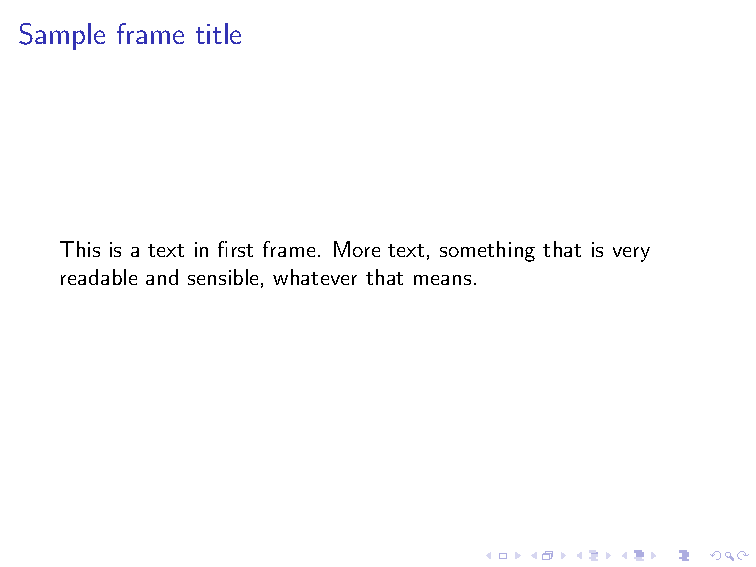
\includegraphics{IdentityTheftSlides/xdusek21-IdentityTheft.pdf}


\subsection{Příprava 3 -- Obecná bezpečnost na Internetu}
Příprava na hodinu s tématem \textbf{Obecná bezpečnost na Internetu} je rozdělena do několika částí:
\begin{itemize}
        \setlength{\itemsep}{-3pt}
        \item Specifikace tématu hodiny,
        \item stanovené cíle,
        \item náplň hodiny a časový plán,
        \item nutné pomůcky pro hodinu
        \item text snímků prezentace.
\end{itemize}

\subsubsection{Specifikace tématu hodiny}
Tato hodina se zabývá aspekty obecné bezpečnosti z hlediska základního uživatelského používání internetového prohlížeče a interakce s webem jako takovým. Částečně téma této hodiny navazuje na předchozí hodinu zaměřenou na \textbf{Krádeže identity} - tato hodina se blíže zaměří na speciální případ krádeže identity, a to případ, kdy podvratná stránka napodobuje svým vzhledem vzhled stránky, kterou uživatel zná a věří ji. Tomuto specializované případu se taktéž říká \textit{Phishing}.

\subsubsection{Stanovené cíle}
Student zná a rozumím pojmům \textit{phishing}, \textit{vývojářská konzole} či jen \textit{konzole}, \textit{zdrojový kód}, \textit{http} a \textit{https}. Student umí rozlišit mezi bezpečnou webovou stránkou a stránkou, která se za bezpečnou webovou stránku pouze vydává. Student dovede posoudit, zda je přípustné do konkrétní webové stránky vyplňovat jakékoliv osobní informace. Student zná a umí vysvětlit problémy z hlediska bezpečnosti, které nastávají při využívání stránek bez podpory HTTPS (tedy stránek, které pro přenos informací mezi uživatelem a serverem využívají HTTP). Student ví k čemu slouží v prohlížečí tzv. \textit{vývojářká konzole} a uvědomuje si, rizika, které neuvážené kopírování a vkládání textu do ní může přinášet.

\subsubsection{Náplň hodiny a časový plán}
\indent\textbf{0. -- 3. minuta} - Zápis do třídní knihy. V případě, že výuka probíhá v počítačové učebně, zapnutí počítačů a přihlášení studentů do systému.

\textbf{4. -- 10. minuta} - Lehké představení tématu hodiny a odkázání se na hodinu týkající se \textbf{Krádeže identity}. Vyučující pokládáním otázek zjistí kolik si toho studenti ze zmíněné hodiny pamatují a nasměruje je na takové odpovědi, které povedou k tématu této hodiny. Například se může zeptat: \uv{Jaké si pamatujete, [Jméno Studenta], možné krádeže identit, ke kterým dochází?}, cílem je dovést studenty ke specializovanému případu krádeže identity a to tomu případu, kdy se stránka vydává za jinou, uživateli známou stránku, což je přímo jedno z témat, které budou probrány.

\textbf{11. -- 25. minuta} - Vyučující využívající počítač připojený k Internetu a data projektoru spustí prohlížeč a ukáže studentům co je to vývojářská konzole a jakým způsobem je ji možné otevřít (tedy klávesou F12). Jsou-li studentům k dispozici počítače s nainstalovanými prohlížeči, vyučující jim pokyne, aby si to také ozkoušeli a vyřeší případné problémy studentů, kterým se konzoli nepodaří najít. Na náhodném webu pak studentům ukáže jak se vepsání kódu do konzole na webu projeví - nejprve na jednoduchém příkladu (vyskakovací okénko), potom na složitějším (úprava obsahu stránky). Vysvětlí jim, že tyto změny se projevují pouze u něho v počítači, změny co provede se nezobrazí dalším návštěvníkům stránky. Pro zvídavé studenty pak může zmínit, že jazyk, kterým se konzole ovládá se jmenuje \textit{Javascript} a používá se hojně pro tvorbu webu. 

Studenti pravděpodobně touto dobou již vědí, že webové stránky jsou programovány a že existuje nějaký kód, na základě kterého jsou stránky zobrazovány. Vyučující toto pro jistotu připomene a ukáže studentům, jak je možné zdrojový kód stránek prohlížet (pro většinu prohlížečů klávesová zkratka \texttt{CTRL + U}). Při ukázce zdrojového kódu existující stránky studentům vysvětlí, že zkopírováním zdrojového kódu stránky a souvisejících souborů k sobě na webovou adresu, by došlo k vytvoření opticky shodné kopie webové stránky, která bude ovšem pod kontrolou někoho jiného. Vyučující se pak zeptá studentů, jestli si dovedou představit nějaký \uv{nepříjemný} scenář, ke kterému by mohlo takto dojít. Studenti by měli dojít k tomu, že by někdo mohl takto získávat informace od lidí, kteří si stránku spletou s originálem. Pokud na to studenti nedojdou, vyučující jim toto prozradí.

V tento moment také vyučující studentům popíše správný postup před zadáním jakýchkoliv soukromých či citlivých informací do webových stránek. Uživatel by měl \textbf{vždy} před vyplněním informací do stránky ověřit, že se opravdu nachází na stránce, na které předpokládá, že je. Toto ověření provede zkontrolováním adresního řádku v prohlížeči. Vyučující zmíní, že ne vždy musí být na první pohled zřejmé, že jde o závadnou stránku - velmi často jsou dnes používány názvy podobné názvu originálu. Jako konkrétní případ lze uvést stránku \textit{PayPal.com}, pro kterou existuje spousta podobných webových stránek, které se snaží napodobit originální jméno, aby působily důvěryhodně, například tedy \textit{PayiPal.com}, či \textit{PayPall.com}. Vyučující se dotáže studentů jaký by použili postup, pokud by si nebyli jistí, že jsou opravdu na stránce, na které chtějí být. Tato otázka může vést na vtipnou odpověď ze stran studentů ve způsobu \uv{Vygooglím si tu stránku?}, která bude v tomto případě na místě a pomůže uvolnit atmosféru v hodině.

Dalším vodítkem hodným zmínění je pak to, zda prohlížeč ve svém adresním řádku má před adresou webové stránky text \textit{https://} nebo \textit{http://}. Většina stránek velkých, středních, ale i menších organizací bude mít před adresou právě \textit{https://}. Většina podvodných stránek \textit{https://} mít vůbec nebude, nebo jen velmi krátkodobě. Vyučující vysvětlí studentům, že většina stránek má zájem o to mít \textit{https}, protože komunikace po tomto protokolu je šifrovaná a zaručuje, že po cestě nebude podvržena, napodobena, či zachycena. To znamená například, že při odesílání formuláře s přihlašovacími údaji na stránce bez aktivního \textit{https} spojení, je možné zachytit přihlašovací údaje po cestě mezi uživatelem a webovou stránkou; to na stránkách s aktivním \textit{https} spojením možné není, právě proto, že komunikace je šifrovaná.

\textbf{26. -- 40. minuta} - Vyučující se s využitím oporných snímků prezentace vrátí k vývojářské konzoli, se kterou studenty seznámil dříve v hodině. Na konkrétních případech skriptů, které byly v minulosti využívány k šíření spamu mezi uživateli sociální sítě Facebook, představí scénář, kterým je možné využít vývojářskou konzoli proti nic netušícímu uživateli. Vysvětlí scénář, který spočívá v přesvědčení uživatelů, že když nakopírují kód do své vývojářské konzole, odemknou si prémiovou verzi sociální sítě, která má lepší možnosti než ta stávající. Uživatelé, kteří kód nakopírují do konzole a pak spustí můžou například nevědomě pozvat všechny své přátele k oblíbení si stránky, která patří útočníkovi, nebo můžou kompromitovat část svých citlivých dat. Vyučující představí reálné případy, kdy k podobným situacím došlo a varuje studenty, aby nikdy takto kód do konzole nekopírovali, pokud nevědí co dělá. Bude-li čas a vhodná situace, vyučující může také jako zajímavost zmínit, že Facebook na tuto hrozbu reagoval a nyní při zobrazení vývojářské konzole v prohlížeči varuje uživatele, aby do ní nic nekopírovali.

\textbf{41. -- 45. minuta} - Shrnutí probrané látky a uzavření tématu. Vyučující dá prostor studentům pro otázky.

\subsubsection{Nutné pomůcky pro hodinu}
Pro efektivní realizaci výuky tak, aby bylo dosaženo stanových cílů je potřeba, aby vyučující měl k dispozici počítač připojení k Internetu s data projektorem zobrazujícím obrazovku počítače třídě. Počítač by měl být vybaven dostatečně moderním internetovým prohlížečem, který obsahuje tzv. \textit{vývojářskou konzoli}.

\subsubsection{Text snímků prezentace}
Sem přijdou snímky prezentace k hodině.


\subsection{Příprava 4 -- Časté a zajímavé pojmy ze světa Kybernetické Bezpečnosti}
Příprava na hodinu s tématem \textbf{Časté a zajímavé pojmy ze světa Kybernetické Bezpečnosti} je rozdělena do několika částí:
\begin{itemize}
        \setlength{\itemsep}{-3pt}
        \item Specifikace tématu hodiny,
        \item stanovené cíle,
        \item náplň hodiny a časový plán,
        \item nutné pomůcky pro hodinu
        \item text snímků prezentace.
\end{itemize}

Hodina je strukturována ve smyslu prezentace různých nepřímo souvisejících pojmů, se kterými se i běžný člověk, který s kybernetickou bezpečností nepřijde do styku na dení bázi, často setká. Na začátku hodiny je studentům představen seznam pojmů, které budou v hodině představeny a diskutovány. Následně jsou pak pojmy jeden po druhém postupně představovány, přičemž při každém přejití na nový pojem se vyučující dotazuje třídy, zda se s pojmem již setkali, popř. zda ho někdo ve třídě dokáže zjednodušeně vysvětlit. Tuto hodinu je možné zařadit na začátek celé výuky kybernetické bezpečnosti, kdy poslouží jako motivace studentů ke studiu a věnování se kybernetické bezpečnosti. Zároveň, pokud bude hodina podána vyhovující formou, může sloužit jako velmi lehký úvod do zajímavých aspektů kybernetické bezpečnosti čímž může u studentů získat na popularitě. Další možností řazení hodiny je její umístění na konec vyučovacího roku, jako poslední zrelaxované a odléhčené téma pro třídu, které studentům dá podnět k vlastnímu studiu kybernetické bezpečnosti i dále - například během prázdnin před dalším během předmětu. Řazení na konec roku je výhodné v tom, že studenti již prošli celým předmětem, spoustu podstatných termínu znají a rozumí jim. A tedy je možné probrat v rámci této hodiny i více komplexní a zajímavá témata, popřípadě provést důkladnou diskuzi na téma.

\subsubsection{Specifikace tématu hodiny} 
Hodina se tématicky zabývá vzájemně nepřímo souvisejícími termíny z oblasti kybernetické bezpečnosti. Pojmy probírané v hodině jsou vybrány tak, aby většinu z nich studenti již za svůj život slyšeli a tato hodina jim pomohla tyto termíny správně uchopit. Probírané termíny jsou pak také vybírány na základě jakési \uv{popularity}, neb mají ve studentech vzbudit zvědavost a určitý pocit senzace, mají na ně působit zajímavě a tajemně. Tato konkrétní příprava na hodinu se zabývá tématem útoků v síti internetu DoS a DDoS, sociálním inženýrstvím, anonymním pohybem po Internetu, sítí TOR a \textit{Deep Webem}. Probrán je také termín botnet. V reálné situaci by však tato příprava na hodinu měla být připravena s ohledem na aktuální důležité termíny a události, které se dějí v oblasti kybernetické bezpečnosti dějí v době očekávaného výkladu, aby poskytnuté informace byly dostatečně aktuální a zajímavé.
%excerpt:některými častými útoky na webové aplikace, 

\subsubsection{Stanovené cíle}
Student rozumí pojmům DoS a DDoS útok a dovede vysvětlit rozdíl mezi nimi. Student zná pojem \uv{sociální inženýrství} a uvědomuje si jeho rizika a právní závadnost případné aplikace jeho disciplín. Student ví co je to \textit{TOR} a k čemu slouží. Student ví jakým způsobem je možné přistoupit na tzv. \uv{\textit{Deep Web}}, a co je na něm možné nalézt. Uvědomuje si, že samotný přístup na \textit{Deep web} není trestný, avšak vyhledávání a prohlížení materiálů, které jsou v rozporu se zákony země, ve které žije, může způsobit právní problémy. Student rozumí pojmu botnet a zná nějaké historicky obrovské botnety a jejich roli ve světě. 
%excerpt:Student umí vyjmenovat a bez zabíhání do detailů přiblížit alespoň 2 časté útoky na webové aplikace. 

\subsubsection{Náplň hodiny a časový plán}
\indent\textbf{0. -- 3. minuta} - Zápis do třídní knihy. V případě, že výuka probíhá v počítačové učebně, zapnutí počítačů a přihlášení studentů do systému.

\textbf{4. -- 8. minuta} - Vyučující promítne na data projektoru úvodní snímek prezentace, na kterém jsou pod sebou v seznamu vypsané termíny, o kterých plánuje v hodině mluvit. Pokyne studentům, aby si zběžně přečetli seznam a dá jim na to trochu času. Následně studentům prozradí, že o těchto pojmech budou tuto hodinu mluvit, a že nyní bude číst pojmy jeden po druhém a pokud někdo ve třídě tento pojem již slyšel, zvedne ruku. Vyučující pak na základě počtu rukou, které zůstávají dole detekuje nejméně obecně známý pojem a bude vědět, na který termín si má vyhradit nejvíce, a naopak nejnémě času. Dle situace a času může vyučující pobídnout někoho ze třídy, aby pojem lehce osvětlil zbytku třídy, bude-li chtít.

\textbf{9. -- 35. minuta} - V tomto časovém úseku budou vysvětlovány a diskutovány jednotlivé témata a termíny, kterými se hodina zabývá. V rámci přípravy je to řazeno do jednoho, dlouhého časového úseku, neb se očekává, že vyučující bude pracovat s časem během hodiny dynamicky - dle znalostí třídy, řazení této hodiny a rozsáhlosti diskusí a studentských dotazů k jednotlivým probíraným tématům.

Vyučující začne přepnutím snímku prezentace na snímek o DoS a DDoS útocích. Vysvětlí studentům anglický význam a překlad těchto zkratek (\textit{Denial of Service}, \textit{Distributed Denial of Service}). Vyučující objasní studentům, že tento populární útok je založen na nárazovém mnohonásobném připojení více klientů / instancí klientů na server za účelem vytížení serveru a znemožnění přístupu legitimních klientů. Po vysvětlení základního princpu a významu zkratek se vyučující pokusí společně se třídou dojít metodou pokládání vhodných otázek k zásadnímu rozdílu mezi útoky. Studenti by měli dojít k uvědomění, že \textit{DDoS} útok je založený na větším množství klientů, rozmístěných například po celém světe, kteří naráz provádějí \textit{DoS} útok. Nedojdou-li k tomu studenti sami od sebe, bude jim to vyučujícím prozrazeno.

Plynulým navázáním na tyto často vyskytující se typy útoků se vyučující přesune k další, pro studenty jistě velmi zajímavé oblasti - vyvětlení, jak principielně může probíhat útok, při kterém se útočník na stejné síti (například. wifi) dostane na počítač oběti útoku. Společně s načnutím tohoto tématu se vyučující posune na odpovídající snímek své prezentace. Popíše jeden z možných scénářů, kterým by útok mohl proběhnout, aby studentům principielně přiblížil jak to reálně celé probíhá, proto, aby konkretizoval představu o tom, co to znamená, když se řekne, že \uv{útočníci se hacknuli do počítače [jméno napadeného člověka]}. Bodově půjde o vysvětlení, že útočník si nejprve provede \uv{průzkum} v rámci kterého nějakým způsobem \uv{proskenuje} síť. Skenováním sítě je myšleno zjištění jaká zařízení jsou v síti na jakých adresách. Jakmile zjistí útočník zařízení v síti, skenuje pak přímo jednotlivě ty. Útočník se pokusí zaslat zprávy na konkrétní zařízení a podle způsobů, kterým zařízení odpovídají někdy dokáže určit, jaký operační systém a v jaké verzi na strojích běží, popřípadě někdy i jaké programy. Dalším krokem je pak to, že útočník nalezne způsob, jak operační systém, nebo běžící program zneužít tak, aby mu byl udělen přístup k zařízení. Toto probíhá typicky tak, že vyhledá v databázi známých bezpečnostních problémů problém konkrétního programového vybavení, které běží na zařízeních v síti. Tohoto bezpečnostního problému dále využije k tomu aby zařízení napadl a převzal nad ním kontrolu.

Dále se vyučující posune na snímek prezentace týkající se sociálního inženýrství. Nejprve se studentů zeptá, co si pod tímto pojmem představí, když ho teď slyší, aby získal představu o tom, jak dalece třída ví o co se jedná. Po úvodních námětech z třídy se dostane vyučující k představení tématu sociálního inženýrství. Vysvětlí třídě, že lidé, kteří jsou nazývání sociálními inženýry jsou specialisté v získávání informací o lidech, procesech, firmách a dalších možných entitách. Obvykle jde o cenné informace buď přímo pro ně, nebo pro osobu, pro kterou pracují. K získávání těchto informací využívají různých manipulačních technik a postupů, ve kterých jsou velmi zběhlí. Vysvětlí, že sociální inženýři velmi často využívají toho, že lidé považují spoustu informací za nepodstatnou a bez problému ji mimoděk sdělí okolí. Pro ilustraci toho, jaký dopad mohou mít zdánlivě nepodstatné informace na společnost, nebo profit jednotlivce, sociálního inženýra, představí vyučující příběh nejmenovaného sociálního inženýra z knihy \textit{The Art of Deception}, od Kevina D. Mitnicka, který demonstruje, jakým způsobem jednoduché, bezcenné informace lze využít. V konkrétním případě volal člověk na několik linek bankovní společnosti, aby nejprve zjistil jakým správným způsobem se ve firmě nazývají určité procedury a informace. Pod záminkou psaní knihy zjistil nejprve to, jak se správně říká \textit{identifikátoru obchodníka}, který se používá u americké firmy \textit{CreditChex}, k ověření, že volající co má zájem o informace volá ze správné firmy. Poděkoval za informaci a vytočil číslo banky, ze které dostal identifikátor obchodníka a volal s jinou operátorkou. Té se představil jako zástupce firmy \textit{CreditChex}, který provádí vyhodnocování spokojenosti klientů jejich firmy a vyptal se operátorky na několik otázek zdánlivě souvisejících se zjišťováním její spokojenosti. Mezi tyto otázky vložil dotaz na identifikátor obchodníka, který používají. Operátorka, považující tuto informaci za naprosto bezcennou, bez váhání sociálnímu inženýrovi tuto informaci sdělila. Co efektivně sociální inženýr během těchto dvou hovorů získal pak byla možnost nyní volat do \textit{CreditChex} společnosti a využívat jejich služeb, aniž by za ně musel platit (nemluvě o tom, že běžní smrtelníci k těmto informacím ani přístup jednoduše nezískají).

Další téma hodiny se týká anonymizační sítě \textit{TOR} a přístupu na \textit{Deep Web}. S vysokou pravděpodobností půjde o, pro studenty, nejzajímavější část hodiny. Vyučující se opět posune na snímek a vysvětlí studentům, že v rámci této hodiny nemá v úmyslu vysvětlovat jim, jak anonymizační síť TOR přesně funguje, ale chce jim objasnit k čemu je dobrá, jak ji využívat a co se na ní dá všechno najít. Vyučující třídě představí \textit{TOR} jako způsob, kterým může kdokoliv na Internetu, při správném používání, zakrýt svou identitu, což znamená, že když osoba využívající \textit{TOR} přistoupí na jakoukoliv webovou stránku, nikdo by neměl být schopen detekovat, že se tak stalo, dokonce ani by nemělo být možné zjistit, z jaké země se člověk připojil. Zde také studentům vysvětlí, že toto platí pouze za předpokladu, že studenti nejsou při používání služeb sítě \textit{TOR} připojeni do svých Facebookových, mailových, či jiných účtů, které uchovávají informace o jejich reálné identitě. Následně se studentů zeptá jaké si dovedou představit scénáře, když by uživatel mohl mít zájem na skrytí své identity na Internetu. Dá se očekávat, že studenti přijdou s důvody, které se odkazují na často pochybné, i nelegální chování. Vyučující by je měl nabádat, aby našli i legitimní důvody, proč by člověk chtěl zůstat na Internetu anonymní. Pokud studenti nepřijdou se svými důvody, řekne jim, že například spousta žurnalistů potřebuje zůstat na Internetu při získávání informací, nebo publikování v anonymitě, aby se nestali terčem útoku, pokud budou psát o něčem, co se někomu nebude líbit. Dalšími případy by pak mohli být lidé skrývající se před všude přítomnou personalizovanou reklamou.

Vyučující studentům představí nejjednodušší - avšak nejméně bezpečný způsob, jak využívat \textit{TOR} k anonymnímu prohlížení Internetu - tento fakt nezapomene zmínit. Způsobem připojení se je využití modifikovaného prohlížeče \textit{Firefox}, který se umožňuje připojit k \textit{TOR} síti. IP adresa, ze které pak uživatel navštěvuje weby není jeho vlastní, ale náhodného uzlu připojeného v anonymizační síti. Vyučující studentům vysvětlí výhody a nevýhody anonymního přístupu na Internet prostřednictvím sítě \textit{TOR}. V tento moment studentům také přiblíží pojem \textit{Deep Web}, který referuje na stránky, které nejsou přístupné z běžného Internetu a dostane se k nim člověk pouze pokud je připojen k \textit{TOR} síti. Tyto stránky mají koncovku \texttt{.onion} a běžně mívají, v závislosti na jejich (ne)legalitě i náhodné jméno složené z alfa numerických znaků (tj. znaků a-z a čísel). Vyučující studentům řekne co všechno za stránky se dá nalézt - od obchodů se zbraněmi, drogami či vraždami, až po zcela normální webové stránky, které se pouze z důvodu jakési \uv{senzace} skrývají za \textit{TOR}em. V tento moment je studentům také sděleno, že samotné navštěvování webu přes TOR není nijak trestně závadné, avšak pokud se budou pohybovat po stránkách jejiž obsah je v rozporu s právy v zemi, ve které žijí, můžou být právně postihování, pokud tato skutečnost vyjde najevo. Toto varování patří například ke stránkám, na kterých může docházet k obchodování s drogami, zbraněmi, lidmi, nebo dětskou pornografií.

Posledním tématem k probrání jsou \textit{botnety}. Vyučující opět začne tento blok posunem na nový snímek a dotazem studentů, jestli by někdo z nich dovedl popsat co to botnet je. Výsledkem společné práce vyučujícího se studenty by mělo být uvědomění studentů, že botnet je skupina zařízení, typicky připojených k Internetu, která po nějakém kanálu přijímají pokyny od majitele botnetu. Příkladem příkazu, který může vydat majitel botnetu je, aby se všechny zařízení připojené v botnetu připojovala opakovaně na nějakou webovou stránku. V tento moment se vyučující zeptá, zda to studentům připomíná nějaké z témat o kterém se v této hodině mluvilo. Očekávanou odpovědí jsou DoS a DDoS útoky, přičemž DDoS je více vítaná odpověď, neb díky většímu počtu reálných klientů po světě, jde o distribuovaný útok na dostupnost služby. Dále se vyučující zeptá studentů, jaká všechna zařízení si myslí, že se mohou připojovat do botnetů. Vzhledem k rapidnímu rozvoji fenoménu zvaného \textit{IoT, (Internet of Things)}, je správnou odpovědí i široká odpověď jako \uv{Potenciálně jakékoliv zařízení s připojením na Internet}. Konkrétně to však v době psaní této práce jsou počítače, telefony, notebooky, chytré ledničky a vysavače, auta apod.

\textbf{40. -- 45. minuta} - Zopakování důležitých termínu z probrané hodiny a shrnutí probrané látky.

%Dalším tématem k rychlému probrání je časté téma napadání webových stránek. Vyučující v naprosté rychlosti představí dva přístupy - jeden jehož výsledkem je vložení nežádoucího zdrojového kódu do webových stránek a druhý, který je postaven na prohledávání a práci s připojenou databází k webové stránce takovým způsobem, který autor stránky nezamýšlel. U prvního zmiňovaného útoku vyučující předpokládá, že žáci již vědí, že webové stránky jsou psány za pomocí HTML, CSS a Javascript technologií. Tento předpoklad však ještě ověří. Dojde-li k závěru, že větší část třídy nemá představu o tom, jak webové stránky vznikají a fungují, nemá smysl se útoky na webové aplikace zabývat a tato část bude přeskočena.

%Má-li třída představu o tom, jak webové stránky fungují, vyučující objasní, že první typ útoku se jmenuje XSS, u kterého rozlišujeme dva případy -- \textit{reflektovaný} a \textit{ukládaný}. Rozdíl mezi nimi je způsob, kterým se útočníkův zdrojový kód do stránek dostává. Při reflektovaném útoku ho stránka do sebe vypisuje na základě informací obdržených od uživatele (například z adresy při odesílání formuláře, nebo z vyhledávacího políčka). 





\subsubsection{Nutné pomůcky pro hodinu}
Pro splnění cílů hodiny mimořádně není nutné žádné speciální elektronické vybavení. Celou hodinu je možné odvést a odvykládat ve standardní učebně, avšak vyučující může benefitovat z dostupnosti počítače napojeného na data projektor. Počítač s data projektorem může využít k živým ukázkám vykládané látky a promítání textů a obrázků na snímcích oporné prezentace. Není-li počítač s data projektorem k dispozici, obsah snímků prezentací lze vyměnit za tabuli a fix, popřípadě křídu.

\subsubsection{Text snímků prezentace}
Text přípravy na hodinu.

% SECTION CONCLUSION
\newpage
\section{Závěr}
%Zhodnocení celé práce, zhruba na 1 A4 - still missing







% === REFERENCES & LITERATURE ===
\newpage
\begin{thebibliography}{9}

    \bibitem{malwareUnicornAppretince}
    Selena Larsen: Malware researcher helps teen hackers turn skills into careers,
    \\\textit{http://money.cnn.com/2017/07/12/technology/malware-researcher-helps-teen-hackers}.

    \bibitem{waveRVP}
    Národní Ústav pro Vzdělávání: Přehled vydávání RVP SOV po vlnách,
    \\\textit{http://www.nuv.cz/t/prehled-vydavani-rvp-sov-po-vlnach}.

    \bibitem{presentationPavlaZ}
    ZIELENIECOVÁ, Pavla. \textit{Příprava učitele na výuku. Vzdělávání učitelů.} [online prezentace]. Praha: Katedra didaktiky fyziky, Matematicko-fyzikální fakulta, UK, 2015, [cit. 2017-19-08]. Dostupný z WWW: $<$https://kdf.mff.cuni.cz/vyuka/pedagogika/materialy/2015\%20ZS/8\%20Priprava\\\%20ucitele\%20na\%20vyuku.\%20Legislativni\%20zakotveni\%20ucitele.pdf$>$.

\end{thebibliography}
\end{document}